\chapter{Implementare}

Acest capitol prezintă implementarea practică a algoritmului Gorilla în limbajul Python. Sunt descrise structura proiectului, clasele principale și deciziile de design.

\section{Structura proiectului}

Proiectul este organizat în mai multe module cu responsabilități distincte:

\begin{verbatim}
PROIECT_PROCESAREA_SEMNALELOR/
|-- BitWriter.py              # Scriere la nivel de bit
|-- BitReader.py              # Citire la nivel de bit
|-- timestamp_compression.py  # Delta-of-delta encoding
|-- value_compression.py      # XOR encoding
|-- storage_minimal.py        # Stocare serii univariate
|-- multivariate_storage.py   # Stocare serii multivariate
|-- run.py                    # Script demonstrativ
+-- timeseries/               # Date de test
    |-- data_cpu.csv
    +-- room_climate_location_A.csv
\end{verbatim}

Diagrama dependențelor este prezentată în Figura~\ref{fig:module-deps}.

\begin{figure}[h]
\centering
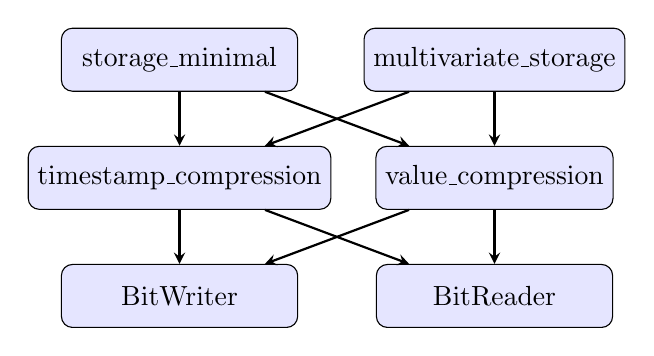
\begin{tikzpicture}[
    module/.style={draw, rectangle, rounded corners, minimum width=3cm, minimum height=0.8cm, align=center, fill=blue!10},
    arrow/.style={->, thick, >=stealth}
]
    % BitWriter and BitReader at the bottom
    \node[module] (bw) at (0,0) {BitWriter};
    \node[module] (br) at (4,0) {BitReader};

    % Compression modules
    \node[module] (ts) at (0,1.5) {timestamp\_compression};
    \node[module] (val) at (4,1.5) {value\_compression};

    % Storage modules
    \node[module] (storage) at (0,3) {storage\_minimal};
    \node[module] (multi) at (4,3) {multivariate\_storage};

    % Dependencies
    \draw[arrow] (ts) -- (bw);
    \draw[arrow] (ts) -- (br);
    \draw[arrow] (val) -- (bw);
    \draw[arrow] (val) -- (br);
    \draw[arrow] (storage) -- (ts);
    \draw[arrow] (storage) -- (val);
    \draw[arrow] (multi) -- (ts);
    \draw[arrow] (multi) -- (val);
\end{tikzpicture}
\caption{Diagrama dependențelor între module}
\label{fig:module-deps}
\end{figure}

\section{Operații pe biți: BitWriter și BitReader}

\subsection{Provocarea}

Python nu oferă acces direct la nivel de bit. Tipul de date fundamental este \texttt{byte} (8 biți). Pentru a implementa compresia Gorilla, avem nevoie să:
\begin{itemize}
    \item Scriem secvențe de biți de lungime arbitrară (1, 5, 7, 12 biți etc.);
    \item Citim aceleași secvențe înapoi;
    \item Gestionăm eficient alinierea la granițe de byte.
\end{itemize}

\subsection{Clasa BitWriter}

\texttt{BitWriter} gestionează scrierea bit-cu-bit într-un buffer de bytes:

\begin{lstlisting}[caption={Structura clasei BitWriter}, label={lst:bitwriter}]
class BitWriter:
    __slots__ = ("_buf", "_cur", "_nbits")

    def __init__(self):
        self._buf = bytearray()  # Bytes completi
        self._cur = 0            # Byte partial in lucru
        self._nbits = 0          # Biti scrisi in _cur (0-7)
\end{lstlisting}

Atributul \texttt{\_\_slots\_\_} este utilizat pentru eficiență: elimină dicționarul implicit al obiectului, reducând consumul de memorie și accelerând accesul la atribute.

\subsubsection{Metoda write\_bit}

Scrierea unui singur bit:

\begin{lstlisting}[caption={Metoda write\_bit}, label={lst:writebit}]
def write_bit(self, bit: int) -> None:
    # Shiftam bitii existenti si adaugam noul bit
    self._cur = (self._cur << 1) | (bit & 1)
    self._nbits += 1

    if self._nbits == 8:
        # Byte complet: il mutam in buffer
        self._buf.append(self._cur & 0xFF)
        self._cur = 0
        self._nbits = 0
\end{lstlisting}

Biții sunt scriși în ordine \textbf{MSB-first} (Most Significant Bit first): bitul cel mai semnificativ este scris primul.

\subsubsection{Metoda write\_bits}

Scrierea unei secvențe de $n$ biți:

\begin{lstlisting}[caption={Metoda write\_bits}, label={lst:writebits}]
def write_bits(self, x: int, n: int) -> None:
    if n == 0:
        return
    if x.bit_length() > n:
        x = x & ((1 << n) - 1)  # Pastram doar n biti

    for i in range(n - 1, -1, -1):
        bit = (x >> i) & 1
        self._cur = (self._cur << 1) | bit
        self._nbits += 1
        if self._nbits == 8:
            self._buf.append(self._cur & 0xFF)
            self._cur = 0
            self._nbits = 0
\end{lstlisting}

\subsubsection{Reprezentarea în complement față de 2}

Pentru numere cu semn, utilizăm funcția de conversie:

\begin{lstlisting}[caption={Conversie la complement fata de 2}, label={lst:twos}]
def to_twos_complement(x: int, num_bits: int) -> int:
    minv = -(1 << (num_bits - 1))  # -2^(n-1)
    maxv = (1 << (num_bits - 1)) - 1  # 2^(n-1) - 1

    if x < minv or x > maxv:
        raise ValueError(f"{x} nu incape pe {num_bits} biti")

    if x < 0:
        x = (1 << num_bits) + x  # 2^n + x

    return x
\end{lstlisting}

\subsection{Clasa BitReader}

\texttt{BitReader} este complementara lui \texttt{BitWriter}:

\begin{lstlisting}[caption={Structura clasei BitReader}, label={lst:bitreader}]
class BitReader:
    __slots__ = ("_data", "_byte_pos", "_bit_pos")

    def __init__(self, data: bytes):
        self._data = data      # Sursa de date
        self._byte_pos = 0     # Indexul byte-ului curent
        self._bit_pos = 0      # Pozitia in byte (0-7)
\end{lstlisting}

\subsubsection{Metoda read\_bit}

\begin{lstlisting}[caption={Metoda read\_bit}, label={lst:readbit}]
def read_bit(self) -> int:
    if self._byte_pos >= len(self._data):
        raise EOFError("End of stream")

    # Extragem bitul de la pozitia curenta (MSB first)
    bit = (self._data[self._byte_pos] >> (7 - self._bit_pos)) & 1

    self._bit_pos += 1
    if self._bit_pos == 8:
        self._bit_pos = 0
        self._byte_pos += 1

    return bit
\end{lstlisting}

\section{Compresia timestamp-urilor}

\subsection{Clasa TimestampEncoder}

Encoder-ul menține starea necesară pentru calculul delta-of-delta:

\begin{lstlisting}[caption={Structura TimestampEncoder}, label={lst:tsenc}]
class TimestampEncoder:
    __slots__ = ("_writer", "_prev_timestamp",
                 "_prev_delta", "_count")

    def __init__(self, writer: BitWriter):
        self._writer = writer
        self._prev_timestamp = None
        self._prev_delta = None
        self._count = 0
\end{lstlisting}

\subsubsection{Metoda add\_timestamp}

\begin{lstlisting}[caption={Adaugarea unui timestamp}, label={lst:addts}]
def add_timestamp(self, timestamp: int) -> None:
    if self._count == 0:
        # Primul timestamp: scriem complet (64 biti)
        self._writer.write_i64(timestamp)
        self._prev_timestamp = timestamp
        self._count = 1
        return

    delta = timestamp - self._prev_timestamp

    if self._count == 1:
        # Al doilea: scriem delta complet
        self._writer.write_i64(delta)
        self._prev_delta = delta
        self._count = 2
        return

    # De la al treilea: delta-of-delta
    dod = delta - self._prev_delta
    self._encode_delta_of_delta(dod)

    self._prev_timestamp = timestamp
    self._prev_delta = delta
    self._count += 1
\end{lstlisting}

\subsubsection{Codarea delta-of-delta}

\begin{lstlisting}[caption={Codarea delta-of-delta}, label={lst:encodedod}]
def _encode_delta_of_delta(self, dod: int) -> None:
    if dod == 0:
        self._writer.write_bit(0)

    elif -64 <= dod <= 63:
        self._writer.write_bit(1)
        self._writer.write_bit(0)
        self._writer.write_signed(dod, 7)

    elif -256 <= dod <= 255:
        self._writer.write_bits(0b110, 3)
        self._writer.write_signed(dod, 9)

    elif -2048 <= dod <= 2047:
        self._writer.write_bits(0b1110, 4)
        self._writer.write_signed(dod, 12)

    else:
        self._writer.write_bits(0b1111, 4)
        self._writer.write_signed(dod, 32)
\end{lstlisting}

\section{Compresia valorilor}

\subsection{Conversia float $\leftrightarrow$ biți}

Pentru a aplica XOR, convertim valorile \texttt{float64} în reprezentarea lor pe 64 de biți folosind modulul \texttt{struct}:

\begin{lstlisting}[caption={Conversie float-biti}, label={lst:floatbits}]
import struct

def float_to_bits(val: float) -> int:
    # Pack ca double big-endian, unpack ca uint64
    return struct.unpack(">Q", struct.pack(">d", val))[0]

def bits_to_float(bits: int) -> float:
    return struct.unpack(">d", struct.pack(">Q", bits))[0]
\end{lstlisting}

\subsection{Clasa ValueEncoder}

\begin{lstlisting}[caption={Structura ValueEncoder}, label={lst:valenc}]
class ValueEncoder:
    __slots__ = ("_writer", "_prev_value_bits",
                 "_prev_leading", "_prev_trailing", "_count")

    def __init__(self, writer: BitWriter):
        self._writer = writer
        self._prev_value_bits = 0
        self._prev_leading = 255   # Sentinel
        self._prev_trailing = 255
        self._count = 0
\end{lstlisting}

\subsubsection{Metoda add\_value}

\begin{lstlisting}[caption={Adaugarea unei valori}, label={lst:addval}]
def add_value(self, val: float) -> None:
    v_bits = self._float_to_bits(val)

    if self._count == 0:
        self._writer.write_u64(v_bits)
        self._prev_value_bits = v_bits
        self._count = 1
        return

    xor = v_bits ^ self._prev_value_bits

    if xor == 0:
        self._writer.write_bit(0)
    else:
        self._writer.write_bit(1)
        self._encode_xor(xor)

    self._prev_value_bits = v_bits
    self._count += 1
\end{lstlisting}

\subsubsection{Calculul leading/trailing zeros}

\begin{lstlisting}[caption={Calculul zeros}, label={lst:zeros}]
def _encode_xor(self, xor: int) -> None:
    bin_xor = bin(xor)[2:].zfill(64)
    leading = len(bin_xor) - len(bin_xor.lstrip('0'))
    trailing = len(bin_xor) - len(bin_xor.rstrip('0'))

    if leading > 31:
        leading = 31  # Limitam la 5 biti

    meaningful_bits = 64 - leading - trailing
\end{lstlisting}

\subsubsection{Decizia de refolosire a ferestrei}

\begin{lstlisting}[caption={Codarea XOR cu decizie fereastra}, label={lst:xorenc}]
    if (self._prev_leading != 255 and
        leading >= self._prev_leading and
        trailing >= self._prev_trailing):
        # Refolosim fereastra anterioara
        self._writer.write_bit(0)
        m = 64 - self._prev_leading - self._prev_trailing
        self._writer.write_bits(xor >> self._prev_trailing, m)
    else:
        # Fereastra noua
        self._writer.write_bit(1)
        self._writer.write_bits(leading, 5)
        self._writer.write_bits(meaningful_bits - 1, 6)
        self._writer.write_bits(xor >> trailing, meaningful_bits)

        self._prev_leading = leading
        self._prev_trailing = trailing
\end{lstlisting}

\textbf{Notă importantă}: Stocăm \texttt{meaningful\_bits - 1} pe 6 biți. Aceasta permite reprezentarea valorilor 1-64 ca 0-63, deoarece când XOR $\neq 0$, există cel puțin un bit semnificativ.

\section{Stocare pentru serii multivariate}

\subsection{Clasa MultiVariateBlock}

Un bloc multivariat gestionează mai multe variabile cu același stream de timestamp-uri:

\begin{lstlisting}[caption={Structura MultiVariateBlock}, label={lst:mvblock}]
class MultiVariateBlock:
    def __init__(self, variable_names: List[str]):
        self._var_names = list(variable_names)
        self._writer = BitWriter()
        self._ts_encoder = TimestampEncoder(self._writer)

        # Un ValueEncoder pentru fiecare variabila
        self._val_encoders = {
            name: ValueEncoder(self._writer)
            for name in self._var_names
        }
        self._count = 0
\end{lstlisting}

\subsection{Adăugarea unui punct multivariat}

\begin{lstlisting}[caption={Adaugarea unui punct multivariat}, label={lst:addmv}]
def add(self, timestamp: int, values: Dict[str, float]):
    # 1. Encodam timestamp-ul O SINGURA DATA
    self._ts_encoder.add_timestamp(timestamp)

    # 2. Encodam fiecare valoare in encoder-ul dedicat
    # IMPORTANT: ordinea trebuie sa fie constanta!
    for name in self._var_names:
        self._val_encoders[name].add_value(values[name])

    self._count += 1
\end{lstlisting}

Ordinea deterministă a variabilelor este esențială: la decodare trebuie să citim valorile în aceeași ordine în care au fost scrise.

\section{Organizarea în blocuri}

Seriile temporale sunt organizate în blocuri de durată fixă (implicit 2 ore = 7.200.000 ms):

\begin{lstlisting}[caption={Gestionarea blocurilor}, label={lst:blocks}]
class MultiVariateSeries:
    def insert(self, timestamp: int, values: Dict[str, float]):
        if self._open_block is None:
            self._create_new_block(timestamp)
        elif timestamp >= self._open_block.start + self._duration:
            self._close_current_block()
            self._create_new_block(timestamp)

        self._open_block.add(timestamp, values)

    def _create_new_block(self, timestamp: int):
        # Aliniem la granita de bloc
        aligned = (timestamp // self._duration) * self._duration
        self._open_block = MultiVariateBlock(self._var_names)
\end{lstlisting}

Alinierea la granița blocului asigură că blocurile consecutive au timestamp-uri de start predictibile, facilitând căutarea în date.

\section{Considerații de performanță}

\subsection{Utilizarea \_\_slots\_\_}

Toate clasele utilizează \texttt{\_\_slots\_\_} pentru:
\begin{itemize}
    \item Reducerea consumului de memorie (fără \texttt{\_\_dict\_\_});
    \item Acces mai rapid la atribute;
    \item Protecție contra erorilor de tip (atribute nedeclarate).
\end{itemize}

\subsection{Evitarea alocărilor în bucla principală}

Metodele de codare evită crearea de obiecte noi în buclele frecvente. Valorile intermediare sunt stocate în variabile de instanță pre-alocate.

\subsection{Buffer pre-alocat}

\texttt{BitWriter} poate primi o capacitate inițială pentru a evita realocări frecvente:

\begin{lstlisting}
def __init__(self, initial_capacity: int = 0):
    self._buf = bytearray()
    if initial_capacity > 0:
        self._buf.extend(b"\x00" * initial_capacity)
        del self._buf[:]  # Golim, dar pastram capacitatea
\end{lstlisting}